\chapter{Loss Function, Optimization, and Advanced Classical Methods}
\lecture{2}{12 Sep. 16:30}{}
\section{Loss function}
\subsection{About the \(x\)-axis of the graph}
Note that in the graph of loss function, the \(x\)-axis is the \textit{margin}, which is \(\hat{y}y \), where \(y\) is the real label and \(\hat{y} \) is the label predicted by the model. Margin is used to estimate our cofidence in the prediction. Because our model generates a score to represent its confidence in the prediction, and in the classic binary classification problem, the label is \(\left\{ -1, 1 \right\} \), so the sign of \(\hat{y} y\) means the predicted label, and \(\vert \hat{y}  \vert \) is the confidence of the prediction. If it predicts something wrong with high confidence, then the loss function will return high value.   
\subsection{Meaning for cross entropy}
The original definition of entropy of a probability distribution \(p\) is 
\[
	H(p) = \mathbb{E} _{x \sim p} [-\log (x)] = -\int p(x) \log p(x) \, \mathrm{dx}. 
\]
The entropy represents how surprised you are to the whole distribution, if some \(x\) with low incidence rate happens, then you will be more surprsied than the one with high incidence rate happen, and note that the grpah of \(y = -\log x\) is as follow:
\begin{figure}[H]
	\centering
	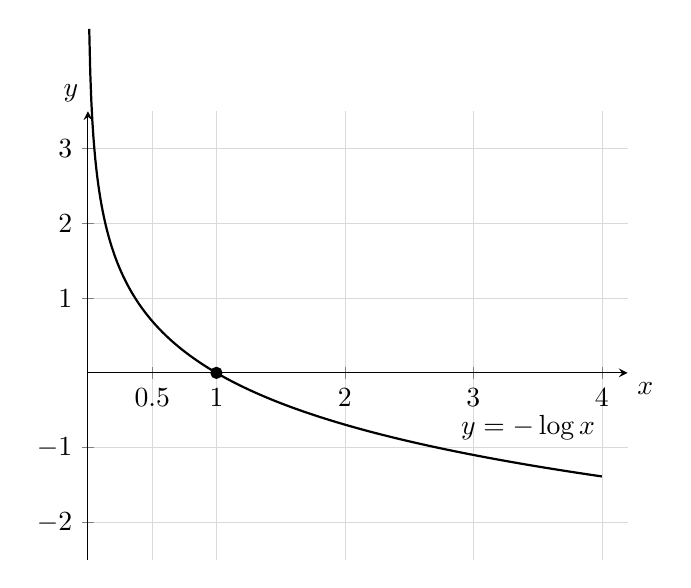
\begin{tikzpicture}
  \begin{axis}[
    axis lines=middle,
    xlabel={$x$}, ylabel={$y$},
    xlabel style={below right},
    ylabel style={above left},
    xmin=0, xmax=4.2,
    ymin=-2.5, ymax=3.5,
    xtick={0,0.5,1,2,3,4},
    ytick={-2,-1,0,1,2,3},
    grid=both,
    grid style={line width=.1pt, draw=gray!20},
    major grid style={line width=.2pt, draw=gray!30},
    samples=500,
    domain=0.01:4,
    clip=false
  ]

    % y = -ln(x)
    \addplot[thick] { -ln(x) } node[pos=0.85, above right] {$y=-\log x$};

    % 幾個標註點 (optional)
    \addplot[only marks, mark=*] coordinates {(1,0)};
  \end{axis}
  
\end{tikzpicture}
	\caption{\(y = -\log x\)}
\end{figure}
Hence, if \(p(x)\) is low, then \(-\log p(x)\) is high, and thus the entropy is well-defined. Hence, we can use entropy to represent the amount of information or the average surprised extent in a probability distribution. 

Now we talk about the cross entropy. Cross entropy can be used to estimate the offset of a predicted distribution \(q\) contrasted to the real distribution \(p\). We will talk about the reason in the following text. The definition of cross entropy of \(p\)(real) and \(q\)(predicted)   is 
\[
	H(p,q) = \mathbb{E}_{x \in p} [- \log q(x)].
\]  
Also, notice that 
\[
	\mathbb{E} _{x \sim p}[-\log q(x)] + \mathbb{E} _{x \sim p} \left[ -\log \frac{p(x)}{q(x)} \right] = \mathbb{E} _{x \sim p} [- \log p(x)],
\]and that 
\[
	\mathbb{E}_{x\sim p}\left[ -\log \frac{p(x)}{q(x)}\right] = \mathbb{E}_{x\sim p}\left[\log \frac{q(x)}{p(x)} \right] \le \log \mathbb{E}_{x\sim p}\left[ \frac{q(x)}{p(x)}\right] = \log 1 = 0  
\] by Jenson's inequality, and thus we know 
\[
	H(p, q) \ge H(p)
\] and the equality holds only when \(p\) is identical to \(q\). Hence, we can use cross entropy to represent if our prediction model is good.

\subsection{Logistic loss function}
If \(\left\{ y_i \right\}_{i=1}^n \) is from a distribution, and our model predicts discrete or continuous labels, then we can use sigmoid function to convert the generated labels to a probability distribution (note that the range of sigmoid function is \([0, 1]\)). Hence, by linking the sigmoid function to the cross entropy, we can estimate if our model is good.

\subsection{Quantile loss}
Quantile loss can help us predict the labels at specific quantile since the optimal point of expected risk function based on quantile loss is at \(q^*\) with \(P(Y < q^*) = \tau \) if we define \(\alpha = \tau \). Hence, if we use this loss funciton to train models, we will set \(q\) to be \(\hat{y} \), and thus we can let the model to predict the label at \(\tau \)-th quantile. In the real training session, we will use some samples to reflect the whole sample space, and then write a approximated \(R(q)\) formula and then use some optimization method like gradient descent to find the optimal "pseudo" \(q\). Now since we know \(\argmin R(q) = q^*\), so we know the \(\tau \)-th quantile's label.     

Let $Y$ be a continuous random variable with cumulative distribution function (CDF) $F_Y$. For a fixed $0 < \tau < 1$, the quantile loss (pinball loss) is defined as
\[
L_\tau(y,q) =
\begin{cases} 
\tau (y-q), & y \ge q, \\
(1-\tau)(q-y), & y < q.
\end{cases}
\]

Define the expected risk:
\[
R(q) = \mathbb{E}[L_\tau(Y,q)] = \int_{-\infty}^{\infty} L_\tau(y,q) \, dF_Y(y).
\]

We want to compute the derivative of $R(q)$ with respect to $q$.

\subsection*{Step 1: Split the integral}
\[
R(q) = \underbrace{\int_{-\infty}^{q} (1-\tau)(q-y) \, dF_Y(y)}_{I_1(q)} + \underbrace{\int_{q}^{\infty} \tau (y-q) \, dF_Y(y)}_{I_2(q)}.
\]

\subsection*{Step 2: Apply Leibniz's rule}
For an integral of the form $\int_{a(q)}^{b(q)} f(y,q) \, dF_Y(y)$, if $f(y,q)$ is differentiable in $q$ and integrable, the derivative is
\[
\frac{d}{dq} \int_{a(q)}^{b(q)} f(y,q) \, dF_Y(y) = f(b(q),q) b'(q) - f(a(q),q) a'(q) + \int_{a(q)}^{b(q)} \frac{\partial f}{\partial q}(y,q) \, dF_Y(y).
\]

\subsubsection*{Integral $I_1(q)$}
\[
I_1(q) = \int_{-\infty}^{q} (1-\tau)(q-y) \, dF_Y(y)
\]
Here $a(q)=-\infty$, $b(q)=q$, $f(y,q) = (1-\tau)(q-y)$, $\frac{\partial f}{\partial q} = 1-\tau$.  
By Leibniz's rule:
\[
\frac{dI_1}{dq} = f(q,q)\cdot 1 - f(-\infty,q)\cdot 0 + \int_{-\infty}^{q} (1-\tau) \, dF_Y(y) = (1-\tau) F_Y(q).
\]

\subsubsection*{Integral $I_2(q)$}
\[
I_2(q) = \int_{q}^{\infty} \tau (y-q) \, dF_Y(y)
\]
Here $a(q)=q$, $b(q)=\infty$, $f(y,q) = \tau(y-q)$, $\frac{\partial f}{\partial q} = -\tau$.  
By Leibniz's rule:
\[
\frac{dI_2}{dq} = f(\infty,q)\cdot 0 - f(q,q)\cdot 1 + \int_{q}^{\infty} (-\tau) \, dF_Y(y) = -\tau (1 - F_Y(q)).
\]

\subsection*{Step 3: Combine derivatives}
\[
\frac{dR}{dq} = \frac{dI_1}{dq} + \frac{dI_2}{dq} = (1-\tau)F_Y(q) - \tau (1 - F_Y(q)) = F_Y(q) - \tau.
\]

\subsection*{Step 4: Find the minimizer}
Setting $\frac{dR}{dq} = 0$ gives
\[
F_Y(q^*) = \tau,
\]
which is exactly the definition of the $\tau$-quantile of $Y$.

\hfill $\square$

\section{Optimization}
\subsection{Why Use the Hessian in Newton's Method?}

Newton's method is a second-order iterative optimization method. Its update rule is:

\[
\theta_{t+1} = \theta_t - H_L(\theta_t)^{-1} \nabla L(\theta_t),
\]

where 
\(\nabla L(\theta_t)\) is the gradient (first derivative) and 
\(H_L(\theta_t)\) is the Hessian (second derivative) of the loss function \(L(\theta)\) at \(\theta_t\).

\subsubsection{1. Intuition}

\begin{itemize}
    \item The gradient \(\nabla L\) tells us \textbf{which direction} to move.
    \item The Hessian \(H_L\) tells us \textbf{how big a step to take} in that direction, based on the local curvature.
\end{itemize}

In other words, the Hessian allows Newton's method to automatically adjust the step size along each direction, unlike gradient descent which requires manually tuned learning rates.

\subsubsection*{2. Advantages of Using the Hessian}

\begin{enumerate}
    \item \textbf{Quadratic convergence:} 
    Near the optimum, Newton's method converges much faster than gradient descent (which converges linearly). Using the Hessian significantly reduces the number of iterations needed.
    
    \item \textbf{Adaptive steps along different directions:} 
    For functions with steep curvature in some directions and flat curvature in others, gradient descent requires careful tuning of the learning rate. 
    Newton's method scales the update according to the curvature automatically:
    \[
    \text{Update step along eigenvector } v_i \sim \frac{1}{\lambda_i} \text{ (eigenvalue of Hessian)}.
    \]
\end{enumerate}

\subsubsection*{3. Why Not Always Use the Hessian?}

\begin{itemize}
    \item \textbf{Computational cost:} Hessian is a \(d \times d\) matrix; storing and inverting it is expensive in high dimensions.
    \item \textbf{Ill-conditioning:} If the Hessian is nearly singular, inversion is unstable.
    \item \textbf{Memory usage:} In deep learning, \(d\) can be tens of thousands or more.
\end{itemize}

\subsubsection*{4. Practical Workarounds}

\begin{itemize}
    \item \textbf{Quasi-Newton methods (BFGS, L-BFGS):} approximate Hessian from past gradients.
    \item \textbf{Gauss-Newton / Levenberg-Marquardt:} specialized for squared-error problems, avoids full Hessian.
    \item \textbf{Hessian-free methods:} use Hessian-vector products to approximate the effect of the Hessian without storing the full matrix.
\end{itemize}

\subsubsection*{Summary}

\[
\text{Hessian is valuable because it provides curvature information, which leads to faster and more stable convergence.}
\]

Even though computing the Hessian can be slow, approximate methods can capture its advantages with lower cost.

\section{Recap: Basic classification}
\section{Advanced classification}
\subsection{Primal and Dual Problems in Optimization and SVM}

\subsubsection*{1. General Optimization Problem}

In optimization, we often want to find the ``best'' value of a function subject to some constraints.  
A general constrained optimization problem is called the \textbf{primal problem}:

\[
\begin{aligned}
\text{minimize} \quad & f(x) \\
\text{subject to} \quad & g_i(x) \le 0, \quad i=1,\dots,m,\\
& h_j(x) = 0, \quad j=1,\dots,p,
\end{aligned}
\]

where
\begin{itemize}
    \item $f(x)$ is the \textbf{objective function} we want to minimize,
    \item $g_i(x) \le 0$ are \textbf{inequality constraints},
    \item $h_j(x) = 0$ are \textbf{equality constraints}.
\end{itemize}

\subsubsection*{2. Lagrangian and Dual Function}

To solve the primal problem, we introduce \textbf{Lagrange multipliers} $\alpha_i \ge 0$ for the inequalities and $\beta_j$ for the equalities.  
The \textbf{Lagrangian} is defined as:

\[
\mathcal{L}(x, \alpha, \beta) = f(x) + \sum_{i=1}^m \alpha_i g_i(x) + \sum_{j=1}^p \beta_j h_j(x)
\]

The \textbf{dual function} is obtained by minimizing the Lagrangian over $x$:

\[
g(\alpha, \beta) = \inf_x \mathcal{L}(x, \alpha, \beta)
\]

Then, the \textbf{dual problem} is:

\[
\begin{aligned}
\text{maximize} \quad & g(\alpha, \beta) \\
\text{subject to} \quad & \alpha_i \ge 0, \quad i=1,\dots,m
\end{aligned}
\]

\textbf{Key points:}
\begin{itemize}
    \item The dual problem provides a lower bound to the primal problem (for minimization).
    \item Sometimes solving the dual is easier than the primal.
    \item Under certain conditions (called \emph{strong duality}), the optimal value of the dual equals that of the primal.
\end{itemize}

\subsubsection*{3. Application to SVM}

For a hard-margin SVM, the primal problem is:

\[
\begin{aligned}
\min_{w,b} \quad & \frac{1}{2} \|w\|^2 \\
\text{subject to} \quad & y_i (w \cdot x_i + b) \ge 1, \quad i=1,\dots,n
\end{aligned}
\]

Here:
\begin{itemize}
    \item $w$ is the weight vector, $b$ is the bias,
    \item $y_i \in \{-1, +1\}$ are the labels,
    \item $x_i$ are the feature vectors,
    \item The constraints ensure that each point is correctly classified with a margin of at least 1.
\end{itemize}

The Lagrangian for this problem is:

\[
\mathcal{L}(w,b,\alpha) = \frac{1}{2}\|w\|^2 - \sum_{i=1}^n \alpha_i \big[y_i (w \cdot x_i + b) - 1\big], \quad \alpha_i \ge 0
\]

Minimizing over $w$ and $b$ leads to the \textbf{dual problem}:

\[
\begin{aligned}
\max_{\alpha} \quad & \sum_{i=1}^n \alpha_i - \frac{1}{2} \sum_{i,j=1}^n \alpha_i \alpha_j y_i y_j (x_i \cdot x_j) \\
\text{subject to} \quad & \sum_{i=1}^n \alpha_i y_i = 0, \quad \alpha_i \ge 0
\end{aligned}
\]

\textbf{Benefits of the dual form:}
\begin{itemize}
    \item Depends only on \textbf{dot products} of data points, allowing the use of kernels.
    \item Often easier to solve when the number of features is large.
    \item The optimal $w$ can be recovered from $\alpha_i$:
    \[
        w = \sum_{i=1}^n \alpha_i y_i x_i
    \]
\end{itemize}

\subsubsection*{4. Summary}

\begin{itemize}
    \item The \textbf{primal problem} is the original optimization problem we want to solve.
    \item The \textbf{dual problem} is derived via Lagrange multipliers and often easier to solve.
    \item In SVMs, the dual problem is particularly useful for kernel methods and large feature spaces.
\end{itemize}

\subsection{Why the Dual Solution Can Match the Primal Optimal Value and Recovering $w$ in SVM}

\subsubsection*{1. Weak and Strong Duality}

Consider a general constrained optimization (primal) problem:

\[
\begin{aligned}
\min_{x} \quad & f(x) \\
\text{subject to} \quad & g_i(x) \le 0, \quad i=1,\dots,m, \\
& h_j(x) = 0, \quad j=1,\dots,p.
\end{aligned}
\]

We define the \textbf{Lagrangian}:

\[
\mathcal{L}(x, \alpha, \beta) = f(x) + \sum_{i=1}^m \alpha_i g_i(x) + \sum_{j=1}^p \beta_j h_j(x), 
\quad \alpha_i \ge 0
\]

and the \textbf{dual function}:

\[
g(\alpha, \beta) = \inf_x \mathcal{L}(x, \alpha, \beta)
\]

Then the dual problem is:

\[
\max_{\alpha, \beta} \quad g(\alpha, \beta) \quad \text{subject to } \alpha_i \ge 0
\]

\textbf{Weak duality:} For any feasible primal $x$ and dual $(\alpha, \beta)$, 

\[
g(\alpha, \beta) \le f(x)
\]

This is always true, so the dual optimum is a \emph{lower bound} of the primal optimum.

\textbf{Strong duality:} If the problem is convex (i.e., $f(x)$ convex, $g_i(x)$ convex, $h_j(x)$ linear) and satisfies some regularity conditions (e.g., Slater's condition), then

\[
\max_{\alpha, \beta} g(\alpha, \beta) = \min_x f(x)
\]

Hence, the \emph{optimal values} of the primal and dual problems are equal.  
However, the \emph{variables} are generally different: the primal variables $x$ are in the original space, while the dual variables $(\alpha, \beta)$ correspond to the constraints.

\subsection*{2. Application to SVM}

For a hard-margin SVM, the primal problem is:

\[
\begin{aligned}
\min_{w,b} \quad & \frac{1}{2} \|w\|^2 \\
\text{subject to} \quad & y_i (w \cdot x_i + b) - 1 \ge 0, \quad i=1,\dots,n
\end{aligned}
\]

The Lagrangian is:

\[
\mathcal{L}(w,b,\alpha) = \frac{1}{2}\|w\|^2 - \sum_{i=1}^n \alpha_i \big[y_i (w \cdot x_i + b) - 1\big], 
\quad \alpha_i \ge 0
\]

To find the dual, we minimize $\mathcal{L}$ with respect to $w$ and $b$:

\[
\frac{\partial \mathcal{L}}{\partial w} = 0 \quad \Rightarrow \quad w = \sum_{i=1}^n \alpha_i y_i x_i
\]

\[
\frac{\partial \mathcal{L}}{\partial b} = 0 \quad \Rightarrow \quad \sum_{i=1}^n \alpha_i y_i = 0
\]

Substituting back, the dual problem becomes:

\[
\begin{aligned}
\max_{\alpha} \quad & \sum_{i=1}^n \alpha_i - \frac{1}{2} \sum_{i,j=1}^n \alpha_i \alpha_j y_i y_j (x_i \cdot x_j) \\
\text{subject to} \quad & \sum_{i=1}^n \alpha_i y_i = 0, \quad \alpha_i \ge 0
\end{aligned}
\]

\subsubsection*{3. Why We Can Recover $w$ from the Dual Solution}

The key is the \textbf{stationarity condition} of the Lagrangian:

\[
\frac{\partial \mathcal{L}}{\partial w} = 0 \quad \Rightarrow \quad w = \sum_{i=1}^n \alpha_i y_i x_i
\]

- This equation comes from setting the derivative of the Lagrangian with respect to the primal variable $w$ to zero.  
- Therefore, once we solve the dual problem and obtain the optimal $\alpha_i^*$, we can recover the optimal $w^*$ as:

\[
w^* = \sum_{i=1}^n \alpha_i^* y_i x_i
\]

Only the **support vectors** have $\alpha_i^* > 0$, so the sum involves only those points that lie on the margin.  
The bias $b$ can then be recovered using any support vector $(x_i, y_i)$:

\[
b = y_i - w^* \cdot x_i
\]

\subsection*{4. Summary}

\begin{itemize}
    \item Duality allows us to transform the primal problem into another problem that may be easier to solve.
    \item Weak duality always holds; strong duality holds for convex problems, including SVM.
    \item In SVM, the dual variables $\alpha_i$ correspond to constraints, not $w$ directly.
    \item $w$ can be recovered from the dual solution via the stationarity condition of the Lagrangian.
\end{itemize}

\subsection{When to use primal problem and dual problem?}
In the p.28 of the lecture slide, it says that if small features and many samples, then use primal problem, while if many features and few samples, then use dual problem. This is because in the primal problem, we have to directly find the best \(w\), which takes \(O(d)\) time to optimize it, where \(d\) is the number of features. As for the dual problem, it takes \(O(n)\) time, where \(n\) is the size of sample set. Note that the time complexity is highly relavant to the number of parameters need to be chose. In the primal problem, we have to select \(d + 1\) parameters \(b, w_1, w_2, \dots , w_d\), while in the dual problem we need to select \(n\) parameters \(\alpha _1, \alpha _2, \dots , \alpha _n\).       

\subsection{Connection between Weak Duality and the Min-Max Inequality}

\subsubsection*{1. Definition of the Dual Function}

For a primal problem:
\[
\min_x f(x) \quad \text{s.t. } g_i(x) \le 0, \, h_j(x) = 0
\]

we define the Lagrangian:
\[
\mathcal{L}(x,\alpha,\beta) = f(x) + \sum_{i} \alpha_i g_i(x) + \sum_j \beta_j h_j(x), \quad \alpha_i \ge 0
\]

The dual function is:
\[
g(\alpha,\beta) = \inf_x \mathcal{L}(x,\alpha,\beta)
\]

\subsubsection*{2. Weak Duality}

By definition of the infimum:
\[
g(\alpha,\beta) = \inf_x \mathcal{L}(x,\alpha,\beta) \le \mathcal{L}(x,\alpha,\beta), \quad \forall x
\]

Now, for any feasible \(x\) (satisfying \(g_i(x)\le 0\) and \(h_j(x)=0\)), the Lagrangian reduces to:
\[
\mathcal{L}(x,\alpha,\beta) = f(x) + \sum_i \alpha_i g_i(x) + \sum_j \beta_j h_j(x) \le f(x)
\]

because \(\alpha_i \ge 0\) and \(g_i(x) \le 0\), and \(h_j(x)=0\).  

Thus, for any feasible \(x\) and any \(\alpha,\beta\ge0\):
\[
g(\alpha,\beta) \le f(x)
\]

This is exactly the **weak duality inequality**.

---

\subsubsection*{3. Min-Max Inequality}

Consider the general min-max problem:
\[
\min_x \max_{\alpha,\beta \ge 0} \mathcal{L}(x,\alpha,\beta) \ge \max_{\alpha,\beta \ge 0} \min_x \mathcal{L}(x,\alpha,\beta)
\]

\begin{itemize}
    \item The left-hand side (LHS) is the \emph{primal perspective}: for each \(x\), pick the worst-case (largest) Lagrangian over \(\alpha,\beta\), then pick the best \(x\) to minimize it.
    \item The right-hand side (RHS) is the \emph{dual perspective}: for each \(\alpha,\beta\), pick the \(x\) that minimizes \(\mathcal{L}\), then pick \(\alpha,\beta\) that maximize this minimum.
\end{itemize}

The inequality
\[
\min_x \max_{\alpha,\beta} \mathcal{L}(x,\alpha,\beta) \ge \max_{\alpha,\beta} \min_x \mathcal{L}(x,\alpha,\beta)
\]
holds \emph{for any function \(\mathcal{L}(x,\alpha,\beta)\)}, not necessarily convex.  

---

\subsubsection*{4. Connecting Weak Duality and Min-Max}

Notice that
\[
\max_{\alpha,\beta \ge 0} \min_x \mathcal{L}(x,\alpha,\beta) = \max_{\alpha,\beta \ge 0} g(\alpha,\beta)
\]

and for feasible \(x\):
\[
\min_x \max_{\alpha,\beta \ge 0} \mathcal{L}(x,\alpha,\beta) = \min_x f(x) = f(x^*) \quad \text{(because feasible \(x\) makes constraints satisfied)}
\]

Here we briefly explain why \(\min _x \max _{ \alpha , \beta \ge 0 } \mathcal{L} (x, \alpha , \beta ) = \min _x f(x) \).  Consider the Lagrangian for a constrained optimization problem:

\[
\mathcal{L}(x, \alpha, \beta) = f(x) + \sum_{i=1}^m \alpha_i g_i(x) + \sum_{j=1}^p \beta_j h_j(x), \quad \alpha_i \ge 0
\]

where \(g_i(x) \le 0\) are inequality constraints and \(h_j(x) = 0\) are equality constraints.

\subsubsection*{1. Maximizing Lagrangian over $\alpha, \beta$}

For a \textbf{feasible point} \(x\) (satisfying \(g_i(x) \le 0\) and \(h_j(x) = 0\)):

\[
\sum_{j=1}^p \beta_j h_j(x) = 0 \quad \text{for any } \beta_j
\]

\[
\sum_{i=1}^m \alpha_i g_i(x) \le 0 \quad \text{because } \alpha_i \ge 0 \text{ and } g_i(x) \le 0
\]

- If \(g_i(x) < 0\), choosing \(\alpha_i > 0\) would decrease \(\mathcal{L}(x,\alpha,\beta)\)  
- Therefore, the maximum over \(\alpha_i \ge 0\) is achieved at \(\alpha_i = 0\)  

Hence, for feasible \(x\):

\[
\max_{\alpha \ge 0, \beta} \mathcal{L}(x, \alpha, \beta) = f(x)
\]

---

\subsubsection*{2. Minimizing over $x$}

\[
\min_x \max_{\alpha \ge 0, \beta} \mathcal{L}(x, \alpha, \beta)
\]

- For infeasible \(x\) (\(g_i(x) > 0\) or \(h_j(x) \neq 0\)), we can make \(\sum_i \alpha_i g_i(x) + \sum_j \beta_j h_j(x)\) arbitrarily large by choosing large \(\alpha_i\) or \(\beta_j\).  
- Hence, infeasible \(x\) will never minimize the max Lagrangian.  
- Only feasible \(x\) contribute, giving \(\max_{\alpha,\beta} \mathcal{L}(x,\alpha,\beta) = f(x)\)

Therefore:

\[
\min_x \max_{\alpha \ge 0, \beta} \mathcal{L}(x, \alpha, \beta) = \min_{x \text{ feasible}} f(x)
\]

---

\subsubsection*{3. Intuition}

- The Lagrange multipliers \(\alpha_i, \beta_j\) act as \emph{penalties} for violating constraints.  
- For feasible \(x\), the penalty terms vanish or are non-positive, so the max over \(\alpha,\beta\) returns \(f(x)\).  
- For infeasible \(x\), the max over \(\alpha,\beta\) blows up, so these points cannot be the minimizer.  

This explains why the min-max formulation over the Lagrangian recovers exactly the primal optimal value.

Then the min-max inequality gives:
\[
\min_{x \text{ feasible}} f(x) = \min_x \max_{\alpha,\beta} \mathcal{L}(x,\alpha,\beta) \ge \max_{\alpha,\beta \ge 0} g(\alpha,\beta)
\]

This is exactly the weak duality statement:
\[
\text{dual optimum} \le \text{primal optimum}
\]

---

\subsubsection*{5. Summary}

\begin{itemize}
    \item The inequality \(g(\alpha,\beta) \le f(x)\) for feasible \(x\) is a pointwise statement.  
    \item The min-max inequality \(\min_x \max_{\alpha,\beta} \mathcal{L} \ge \max_{\alpha,\beta} \min_x \mathcal{L}\) is the global version and directly implies weak duality.  
    \item For convex problems (like SVM), strong duality holds, meaning the inequality becomes equality:
    \[
    \min_x \max_{\alpha,\beta} \mathcal{L}(x,\alpha,\beta) = \max_{\alpha,\beta} \min_x \mathcal{L}(x,\alpha,\beta)
    \]
\end{itemize}
